\appendix

\titleformat{\chapter}[block] % Format for the chapter title
  {\normalfont\huge\bfseries}  % Title font
  {\thechapter}{1em}{}         % Chapter numbering formatting
\titlespacing*{\chapter}{0pt}{-1cm}{1em}  % Adjust the spacing: 0pt for left, -2cm to move up, 1em for after title

\chapter*{Appendix}  % This adds "Appendix" to the ToC but avoids double title
\addcontentsline{toc}{chapter}{Appendix}  % Adds "Appendix" to the ToC manually
\setcounter{section}{0}  % Reset section counter
\renewcommand{\thesection}{\Alph{section}}  % Change section numbering to letters (A, B, C...)
%\vspace{-1.5cm}
\section{Toro test cases}\label{app:toro_test_cases}
\vspace{-0.5cm}
\subsection{Toro test case 1}\label{app:toro_test_case_1}

\begin{figure}[H]
    \centering
    \begin{minipage}{0.45\textwidth}
        \centering
        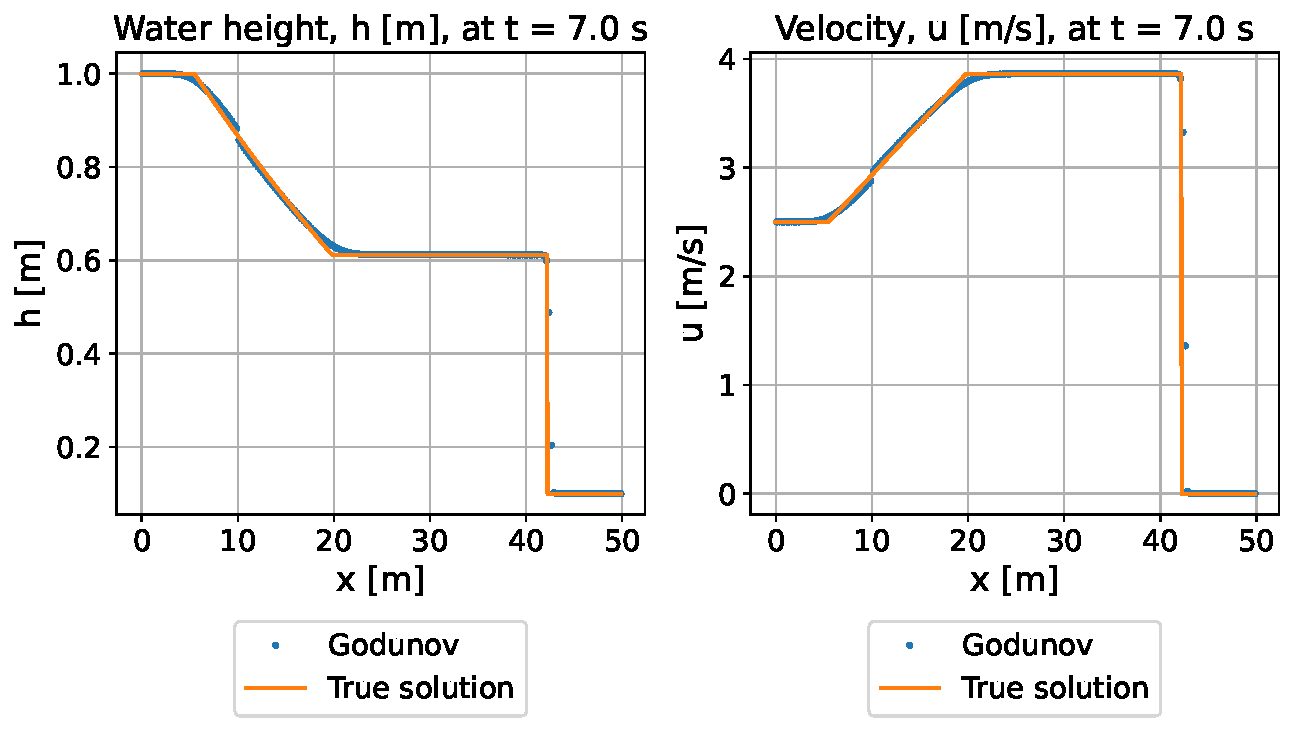
\includegraphics[width=\textwidth]{C:/Users/Matteo/Shallow-Water-Equations/plots/toro_test1_final_GOD.pdf}
        \subcaption{Godunov flux.}
    \end{minipage}%
    \hfill
    \begin{minipage}{0.45\textwidth}
        \centering
        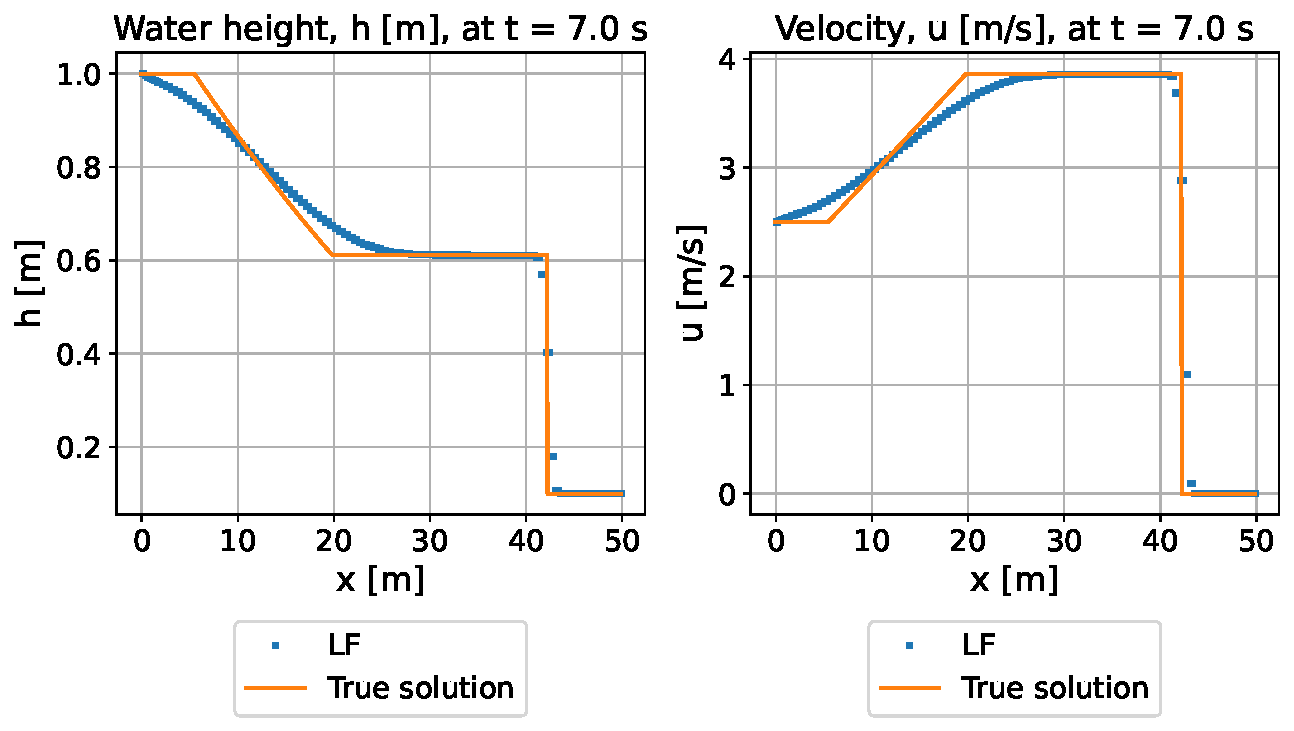
\includegraphics[width=\textwidth]{C:/Users/Matteo/Shallow-Water-Equations/plots/toro_test1_final_LF.pdf}
        \subcaption{LF flux.}
    \end{minipage}

    \vspace{0.5cm} % Vertical space between rows
    
    \begin{minipage}{0.45\textwidth}
        \centering
        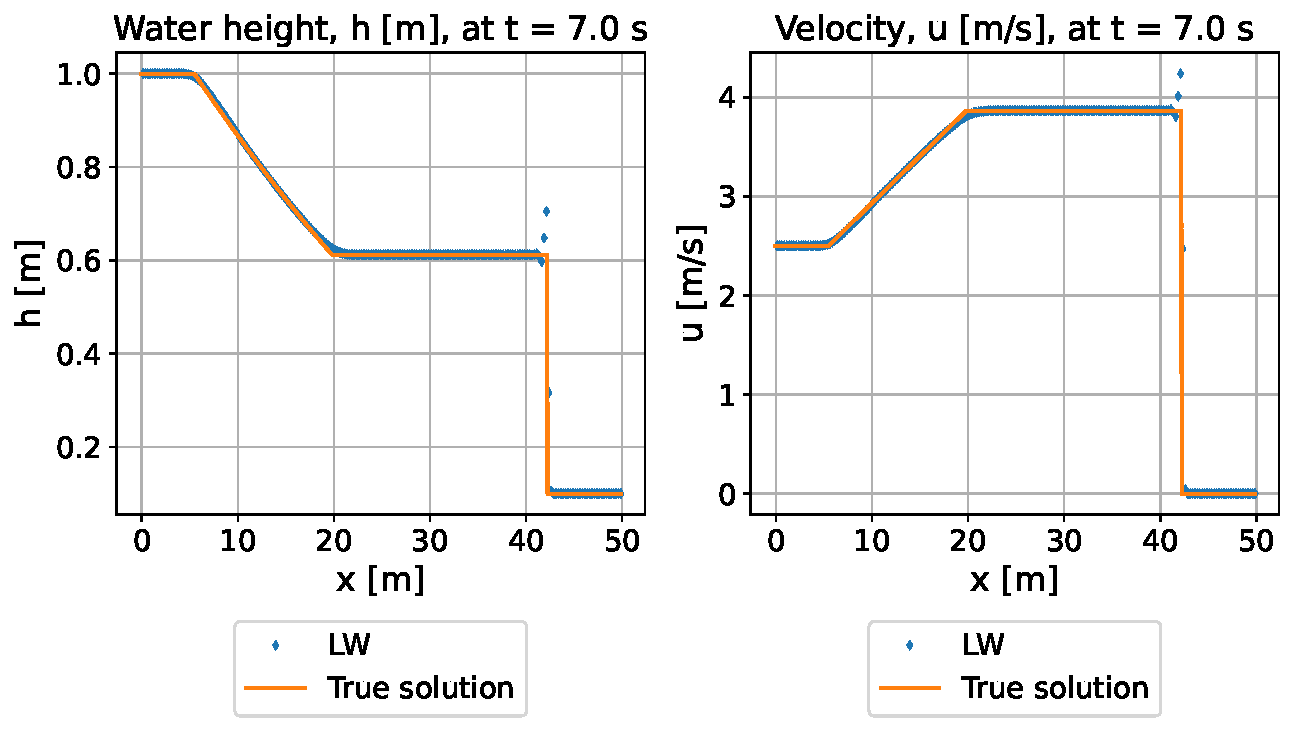
\includegraphics[width=\textwidth]{C:/Users/Matteo/Shallow-Water-Equations/plots/toro_test1_final_LW.pdf}
        \subcaption{LW flux.}
    \end{minipage}%
    \hfill
    \begin{minipage}{0.45\textwidth}
        \centering
        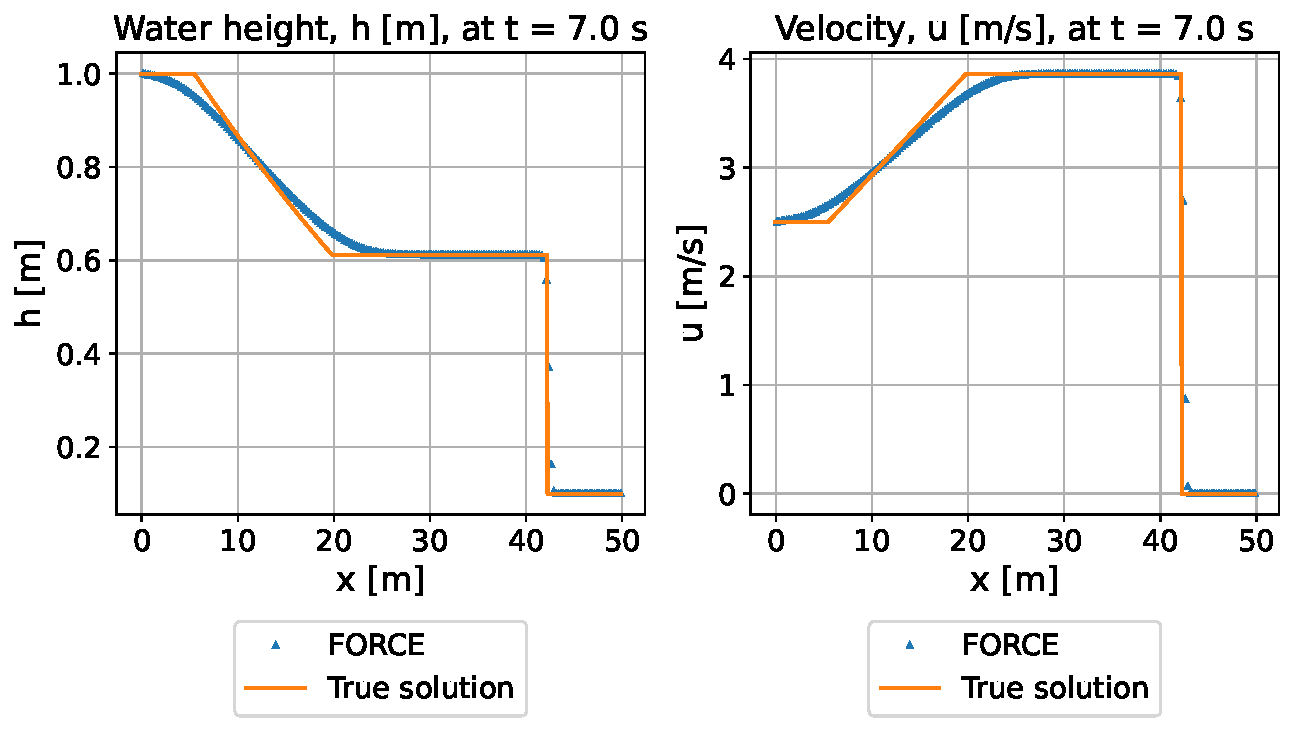
\includegraphics[width=\textwidth]{C:/Users/Matteo/Shallow-Water-Equations/plots/toro_test1_final_FORCE.pdf}
        \subcaption{FORCE flux.}
    \end{minipage}

    \vspace{0.5cm} % Vertical space between rows
    
    \begin{minipage}{0.45\textwidth}
        \centering
        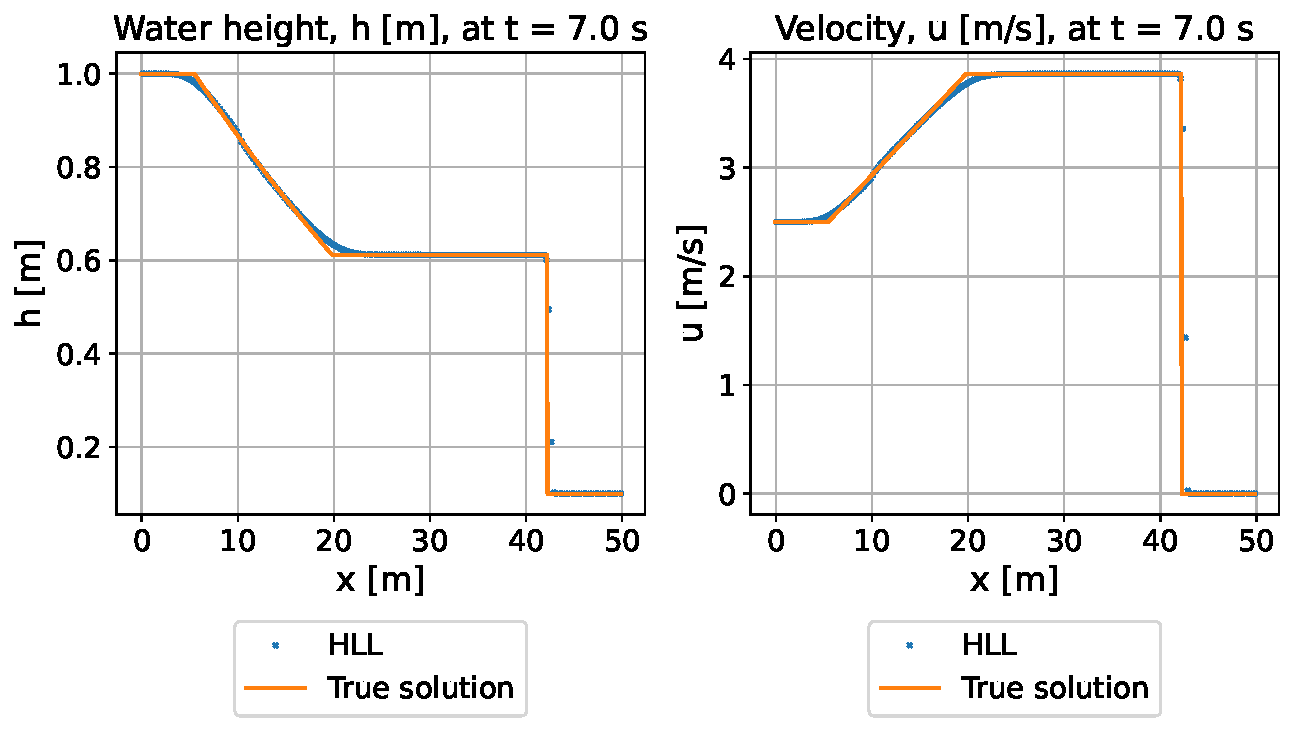
\includegraphics[width=\textwidth]{C:/Users/Matteo/Shallow-Water-Equations/plots/toro_test1_final_HLL.pdf}
        \subcaption{HLL flux.}
    \end{minipage}
    \caption{Comparison of the different fluxes for Toro test case 1.}\label{fig:toro_test1_fluxes}
\end{figure}


\subsection{Toro test case 2}\label{app:toro_test_case_2}

\begin{figure}[H]
    \centering
    \begin{minipage}{0.45\textwidth}
        \centering
        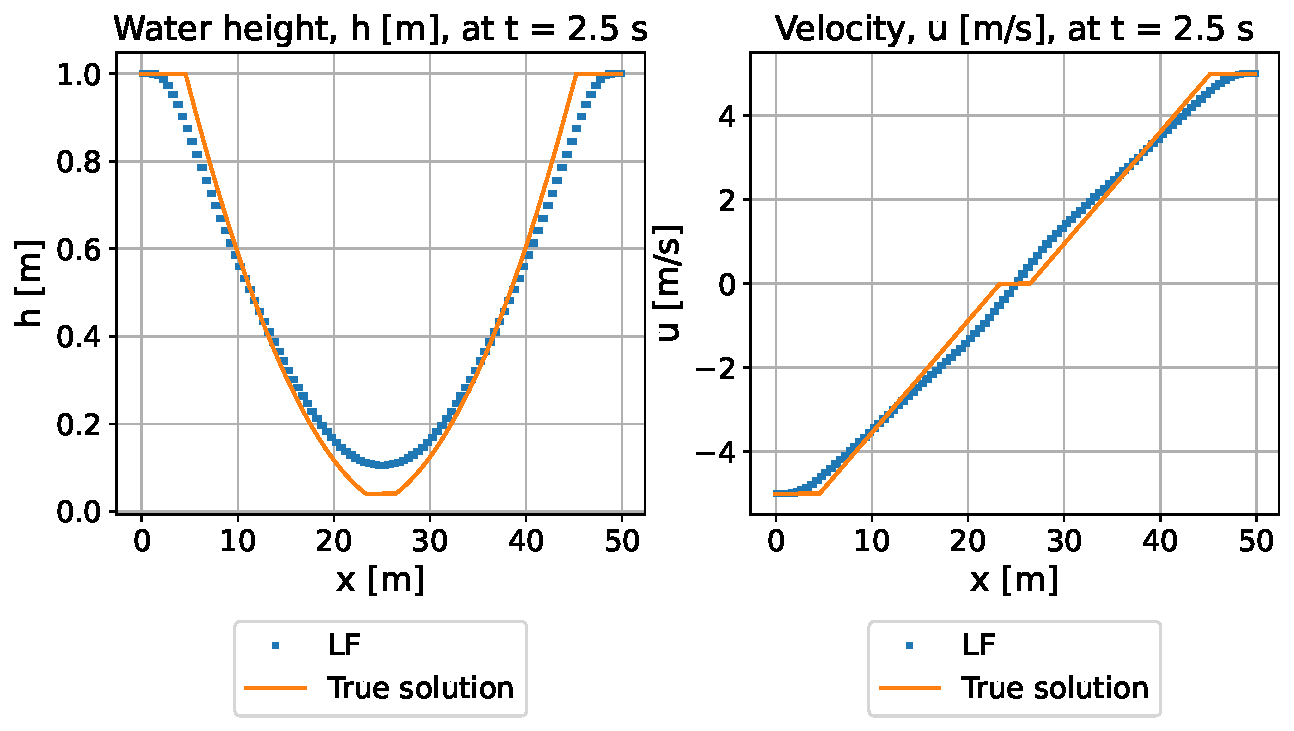
\includegraphics[width=\textwidth]{C:/Users/Matteo/Shallow-Water-Equations/plots/toro_test2_final_LF.pdf}
        \subcaption{LF flux.}
    \end{minipage}%
    \hfill
    \begin{minipage}{0.45\textwidth}
        \centering
        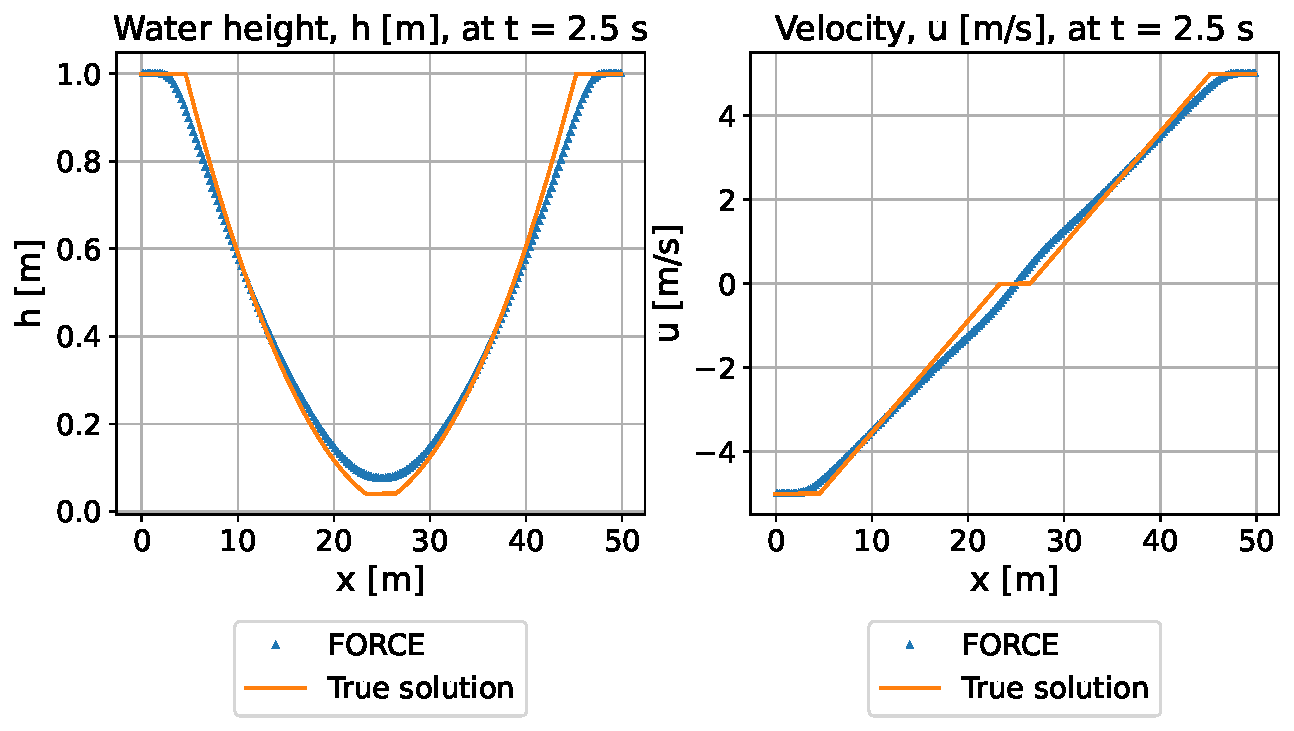
\includegraphics[width=\textwidth]{C:/Users/Matteo/Shallow-Water-Equations/plots/toro_test2_final_FORCE.pdf}
        \subcaption{FORCE flux.}
    \end{minipage}
    
    \vspace{0.5cm} % Vertical space between rows    
    \begin{minipage}{0.45\textwidth}
        \centering
        % Replace with your other figure for HLL
        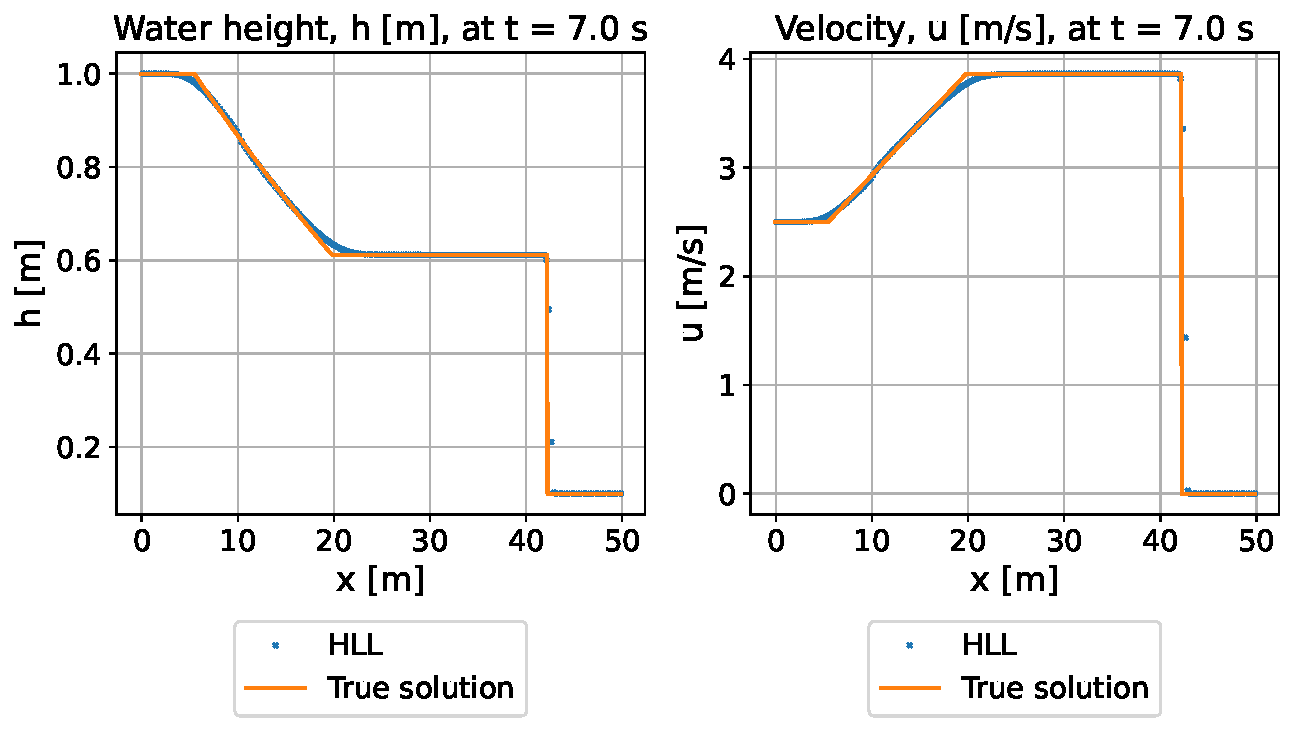
\includegraphics[width=\textwidth]{C:/Users/Matteo/Shallow-Water-Equations/plots/toro_test1_final_HLL.pdf}
        \subcaption{HLL flux.}
    \end{minipage}
    \caption{Comparison of the different fluxes for Toro test case 2.}\label{fig:toro_test2_fluxes}
\end{figure}



\subsection{Toro test case 3}\label{app:toro_test_case_3}
\begin{figure}[H]
    \centering
    \begin{minipage}{0.45\textwidth}
        \centering
        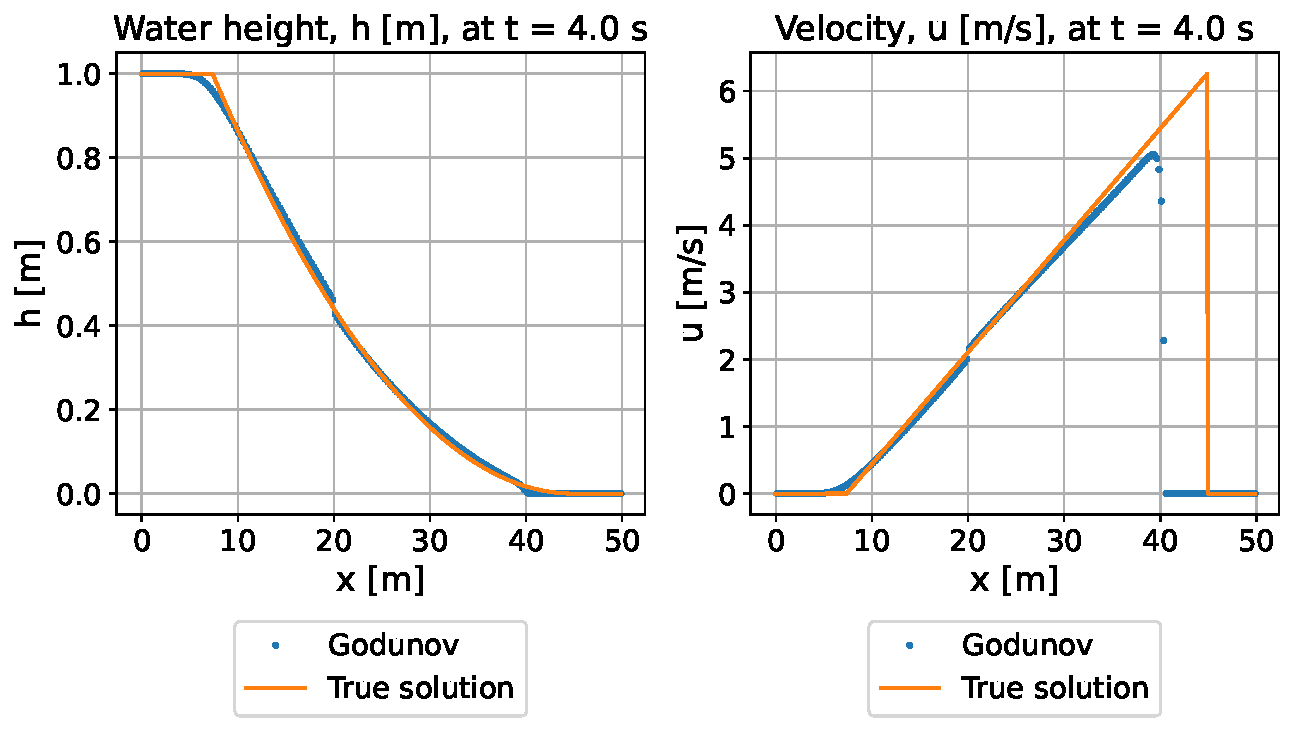
\includegraphics[width=\textwidth]{C:/Users/Matteo/Shallow-Water-Equations/plots/toro_test3_final_GOD.pdf}
        \subcaption{Godunov flux.}
    \end{minipage}%
    \hfill
    \begin{minipage}{0.45\textwidth}
        \centering
        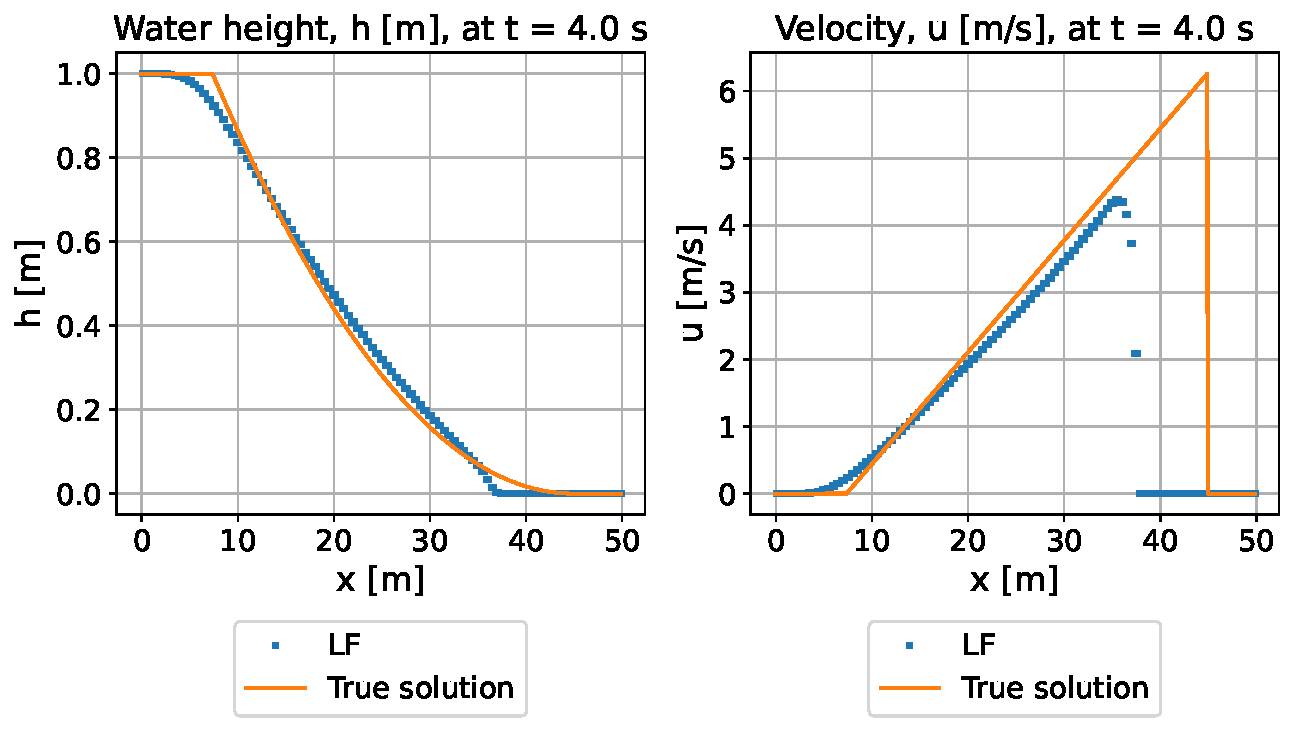
\includegraphics[width=\textwidth]{C:/Users/Matteo/Shallow-Water-Equations/plots/toro_test3_final_LF.pdf}
        \subcaption{LF flux.}
    \end{minipage}
    
    \vspace{0.5cm} % Vertical space between rows
    
    \begin{minipage}{0.45\textwidth}
        \centering
        % Replace with your other figure for LW
        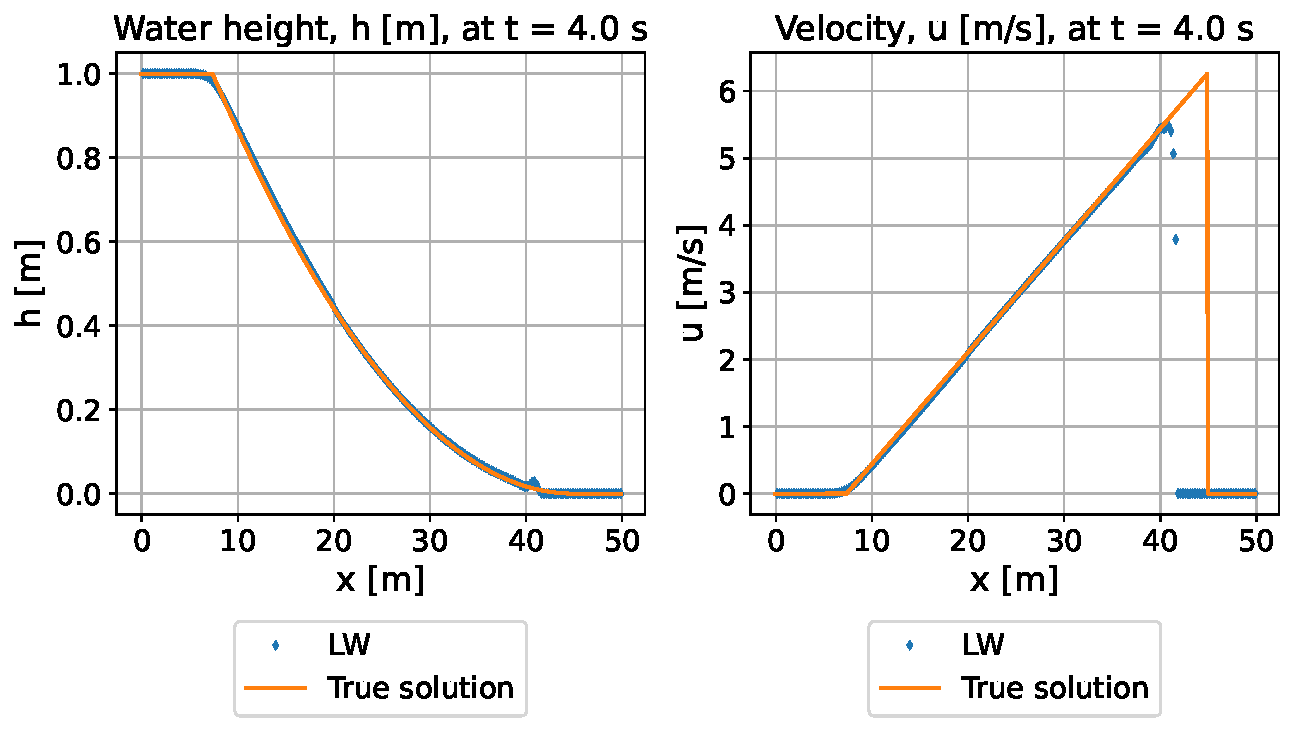
\includegraphics[width=\textwidth]{C:/Users/Matteo/Shallow-Water-Equations/plots/toro_test3_final_LW.pdf}
        \subcaption{LW flux.}
    \end{minipage}%
    \hfill
    \begin{minipage}{0.45\textwidth}
        \centering
        % Replace with your other figure for FORCE
        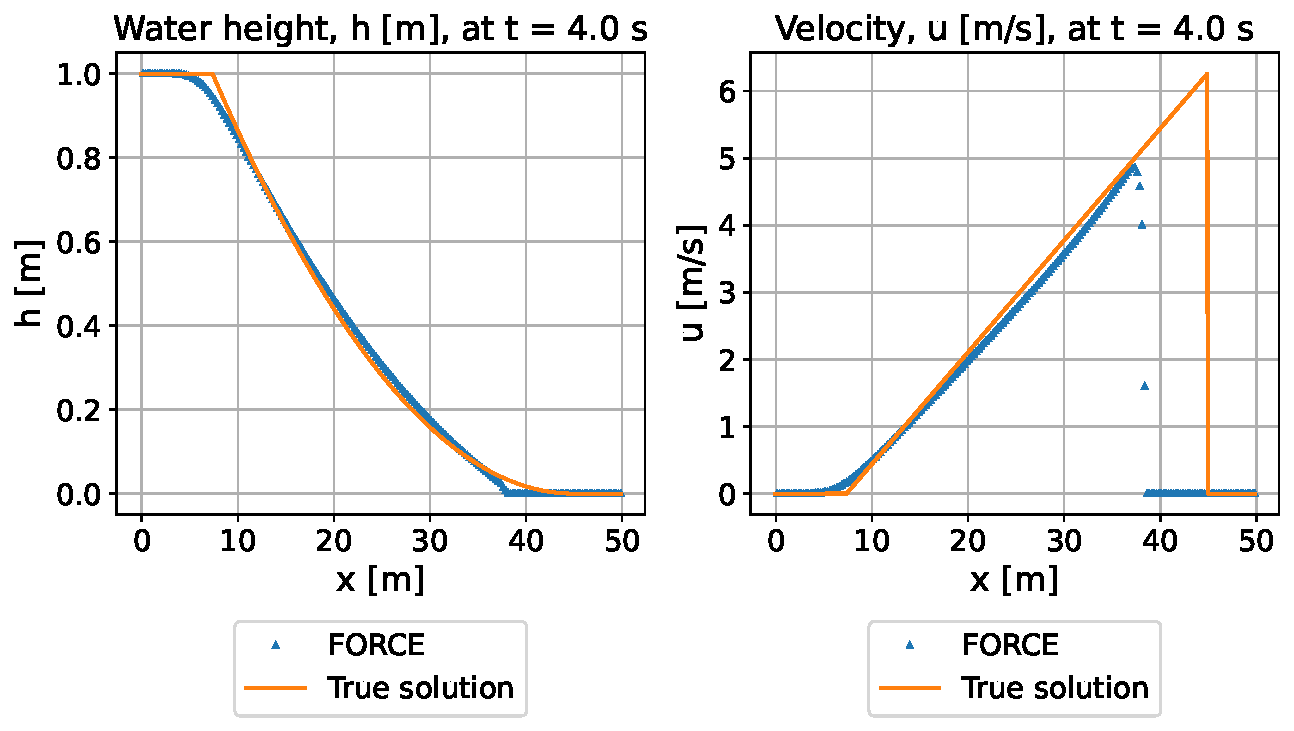
\includegraphics[width=\textwidth]{C:/Users/Matteo/Shallow-Water-Equations/plots/toro_test3_final_FORCE.pdf}
        \subcaption{FORCE flux.}
    \end{minipage}

    \vspace{0.5cm} % Vertical space between rows
    
    \begin{minipage}{0.45\textwidth}
        \centering
        % Replace with your other figure for HLL
        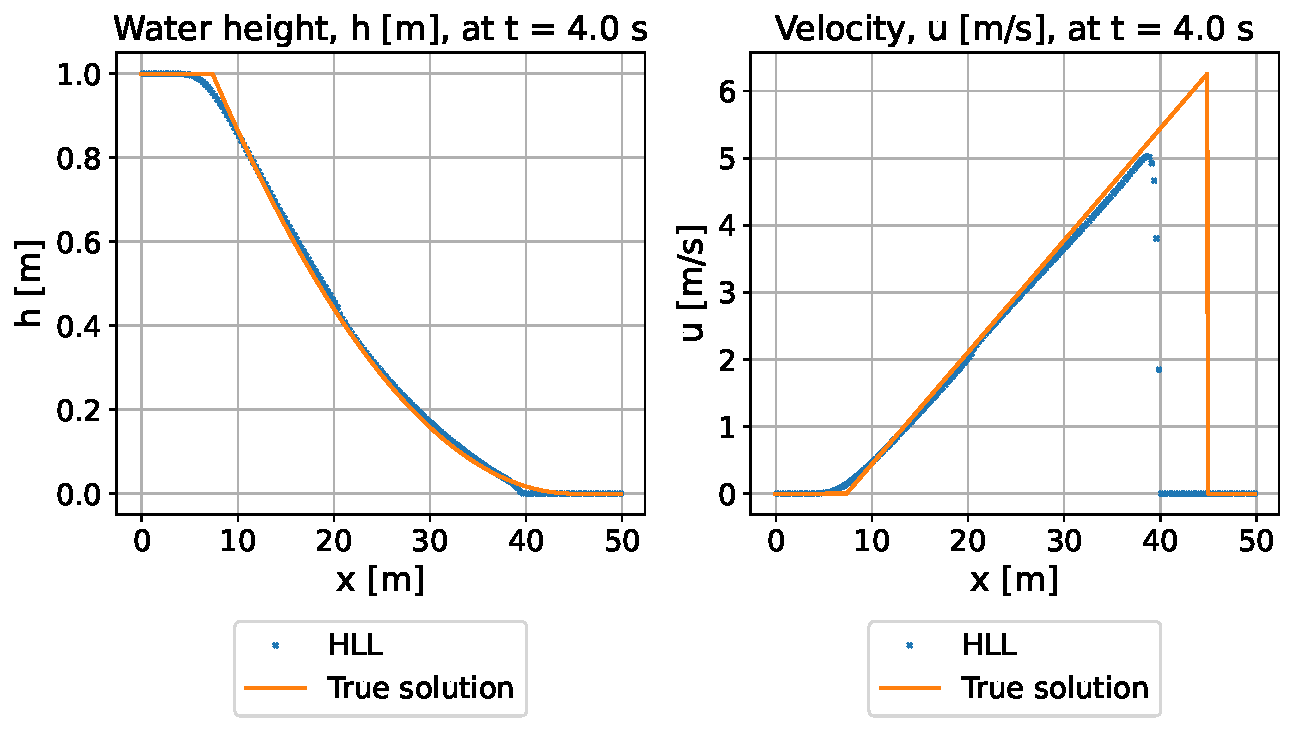
\includegraphics[width=\textwidth]{C:/Users/Matteo/Shallow-Water-Equations/plots/toro_test3_final_HLL.pdf}
        \subcaption{HLL flux.}
    \end{minipage}
    \caption{Comparison of the different fluxes for Toro test case 3.}\label{fig:toro_test3_fluxes}
\end{figure}




\subsection{Toro test case 4}\label{app:toro_test_case_4}
\begin{figure}[H]
    \centering
    \begin{minipage}{0.45\textwidth}
        \centering
        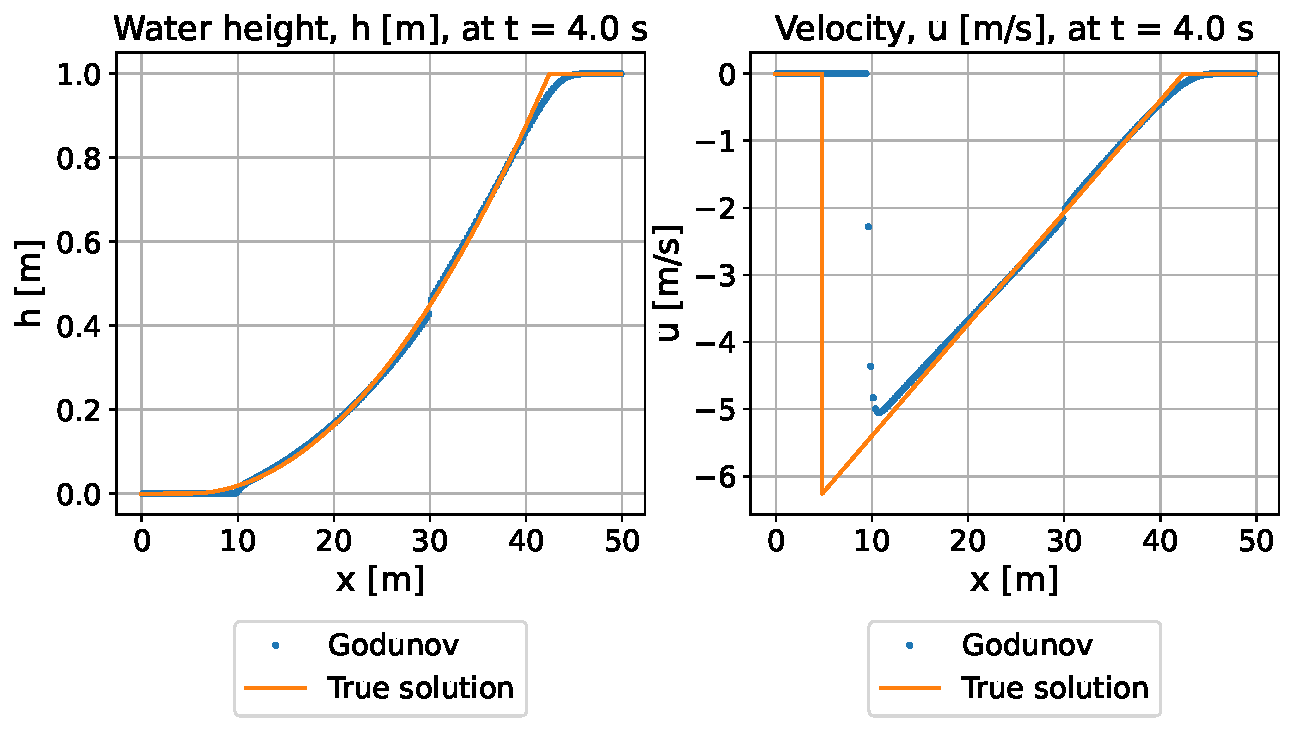
\includegraphics[width=\textwidth]{C:/Users/Matteo/Shallow-Water-Equations/plots/toro_test4_final_GOD.pdf}
        \subcaption{Godunov flux.}
    \end{minipage}%
    \hfill
    \begin{minipage}{0.45\textwidth}
        \centering
        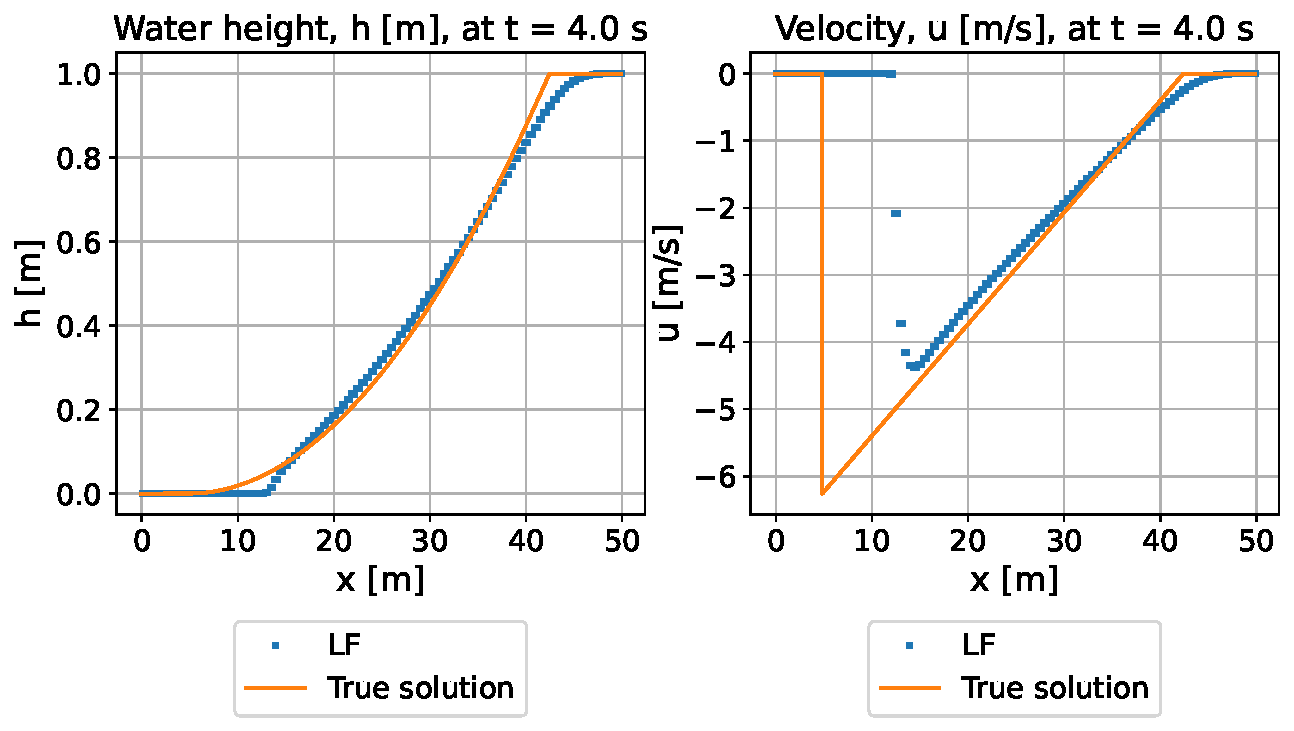
\includegraphics[width=\textwidth]{C:/Users/Matteo/Shallow-Water-Equations/plots/toro_test4_final_LF.pdf}
        \subcaption{LF flux.}
    \end{minipage}
    
    \vspace{0.5cm} % Vertical space between rows
    
    \begin{minipage}{0.45\textwidth}
        \centering
        % Replace with your other figure for LW
        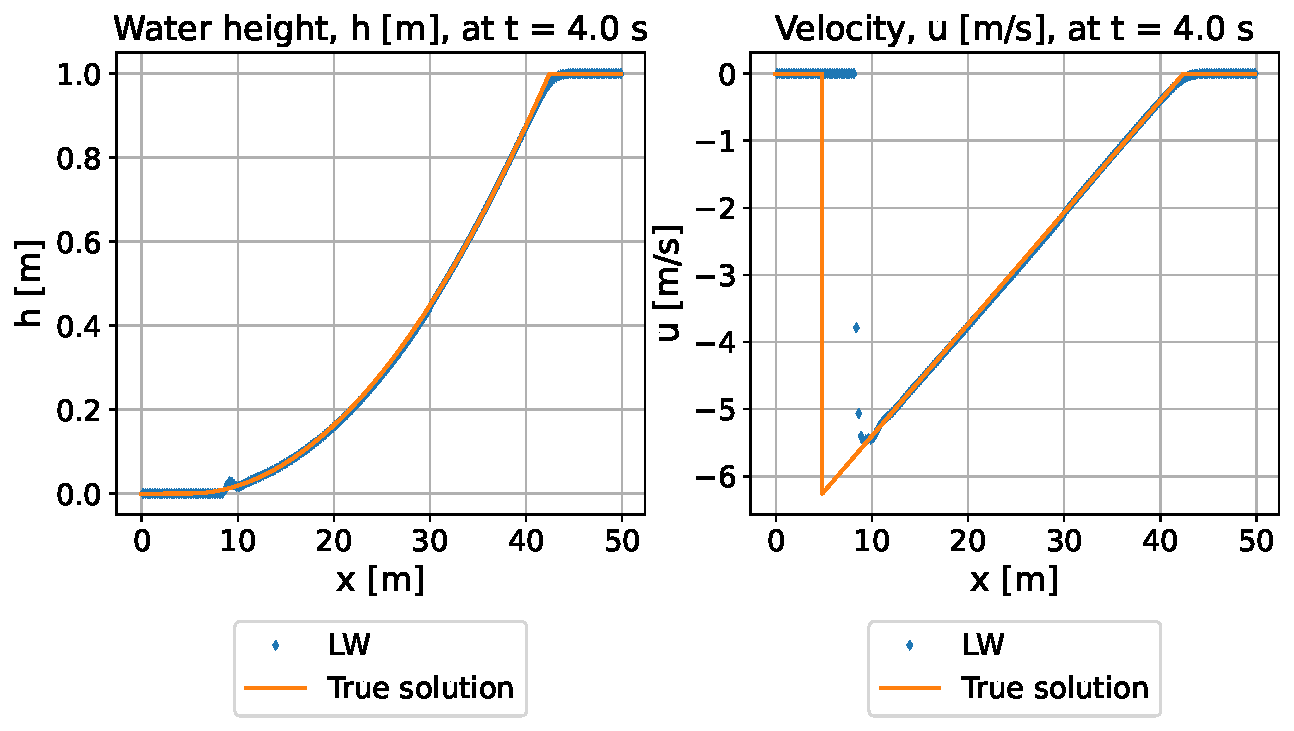
\includegraphics[width=\textwidth]{C:/Users/Matteo/Shallow-Water-Equations/plots/toro_test4_final_LW.pdf}
        \subcaption{LW flux.}
    \end{minipage}%
    \hfill
    \begin{minipage}{0.45\textwidth}
        \centering
        % Replace with your other figure for FORCE
        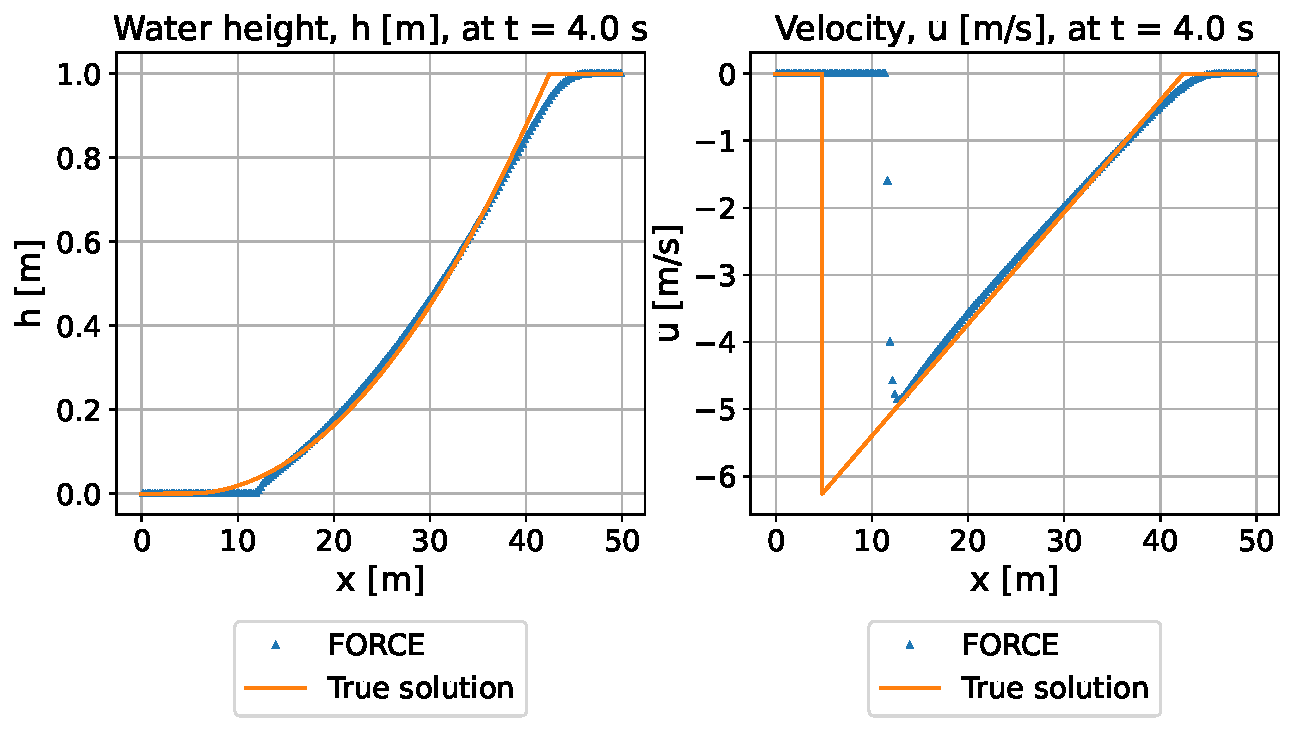
\includegraphics[width=\textwidth]{C:/Users/Matteo/Shallow-Water-Equations/plots/toro_test4_final_FORCE.pdf}
        \subcaption{FORCE flux.}
    \end{minipage}

    \vspace{0.5cm} % Vertical space between rows
    
    \begin{minipage}{0.45\textwidth}
        \centering
        % Replace with your other figure for HLL
        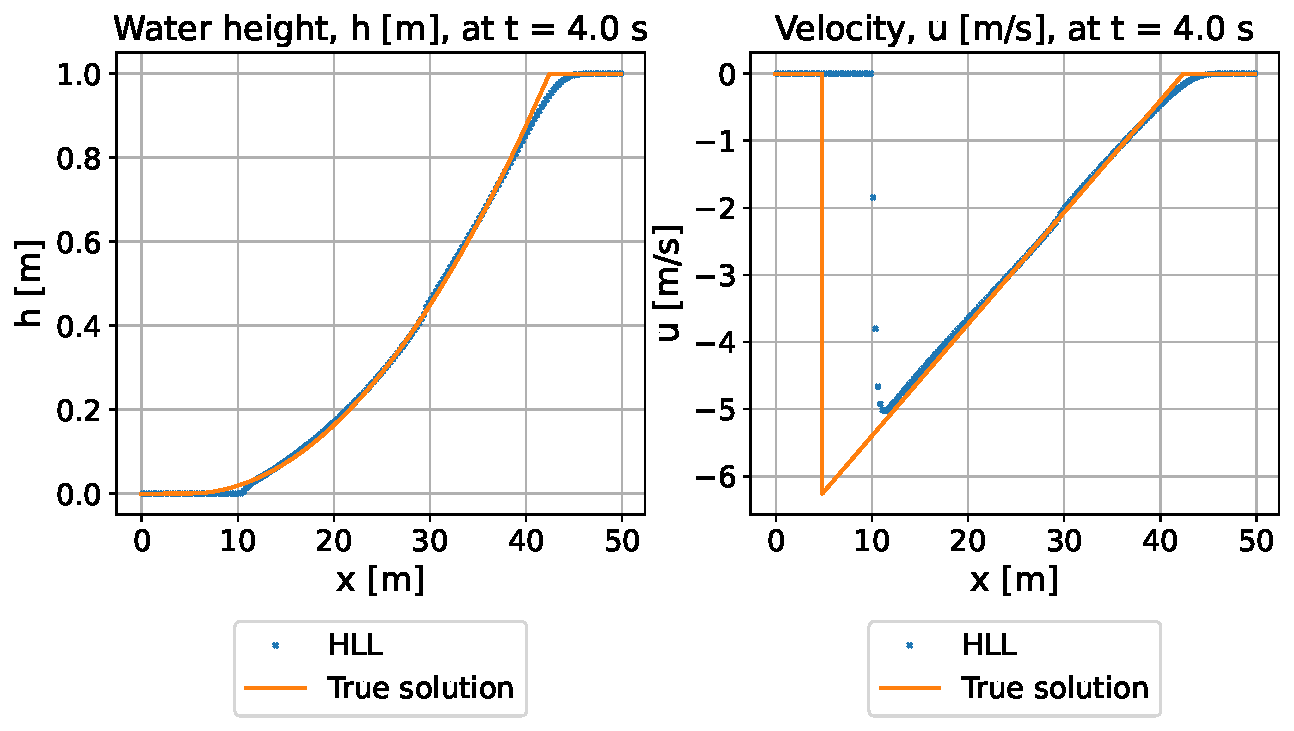
\includegraphics[width=\textwidth]{C:/Users/Matteo/Shallow-Water-Equations/plots/toro_test4_final_HLL.pdf}
        \subcaption{HLL flux.}
    \end{minipage}
    \caption{Comparison of the different fluxes for Toro test case 4.}\label{fig:toro_test4_fluxes}
\end{figure}



\subsection{Toro test case 5}\label{app:toro_test_case_5}

\begin{figure}[H]
    \centering
    \begin{minipage}{0.45\textwidth}
        \centering
        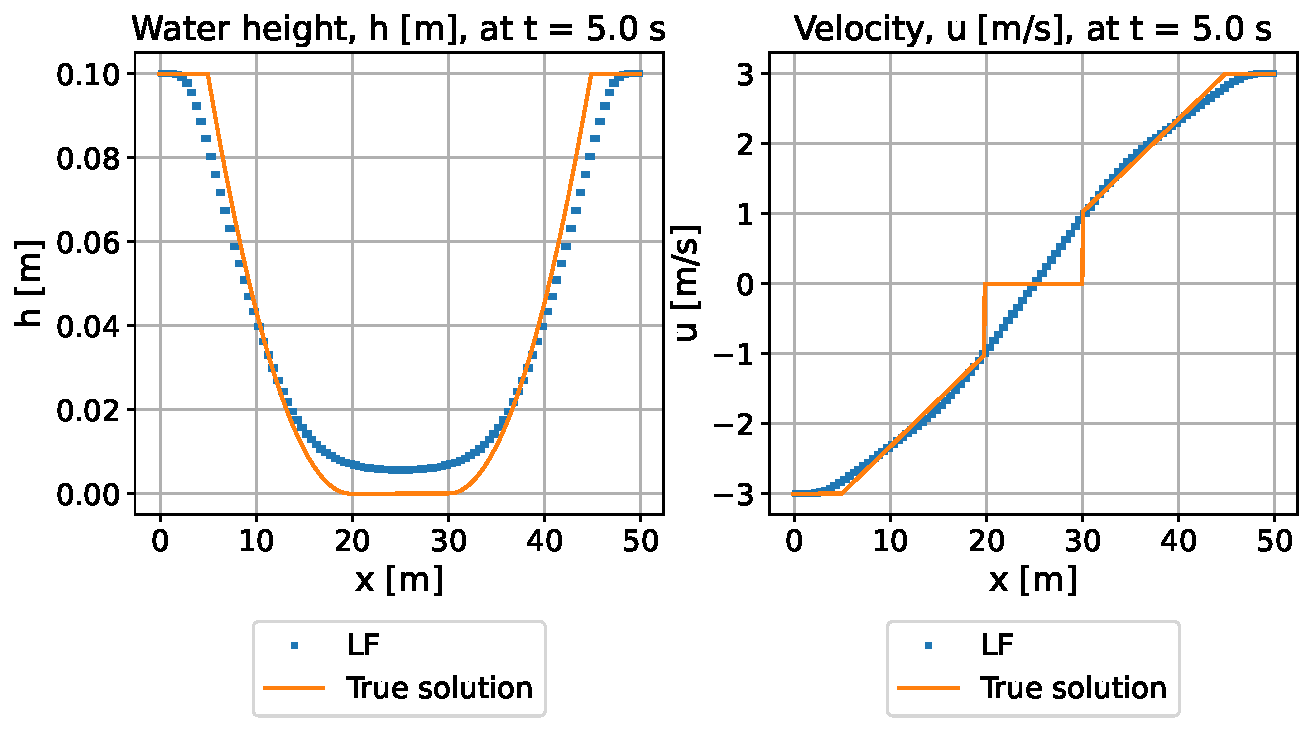
\includegraphics[width=\textwidth]{C:/Users/Matteo/Shallow-Water-Equations/plots/toro_test5_final_LF.pdf}
        \subcaption{LF flux.}
    \end{minipage}%
    \hfill
    \begin{minipage}{0.45\textwidth}
        \centering
        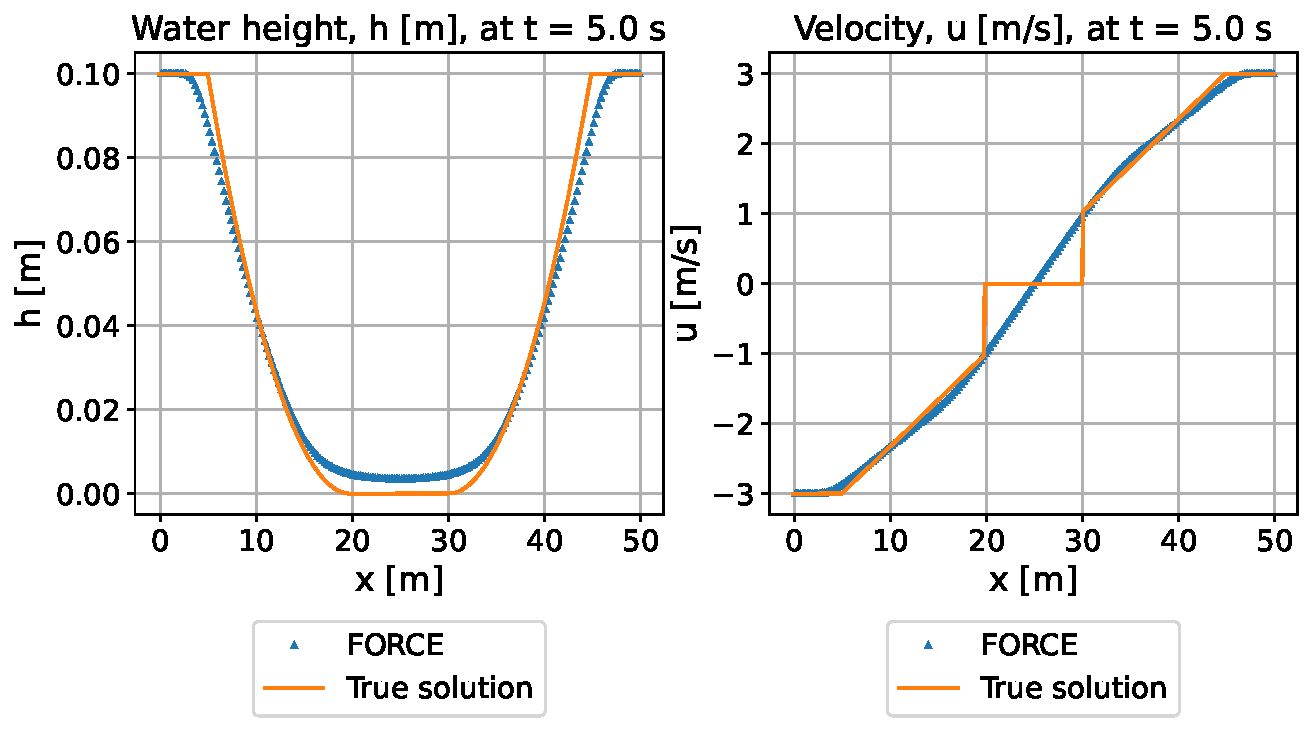
\includegraphics[width=\textwidth]{C:/Users/Matteo/Shallow-Water-Equations/plots/toro_test5_final_FORCE.pdf}
        \subcaption{FORCE flux.}
    \end{minipage}
    
    \vspace{0.5cm} % Vertical space between rows    
    \begin{minipage}{0.45\textwidth}
        \centering
        % Replace with your other figure for HLL
        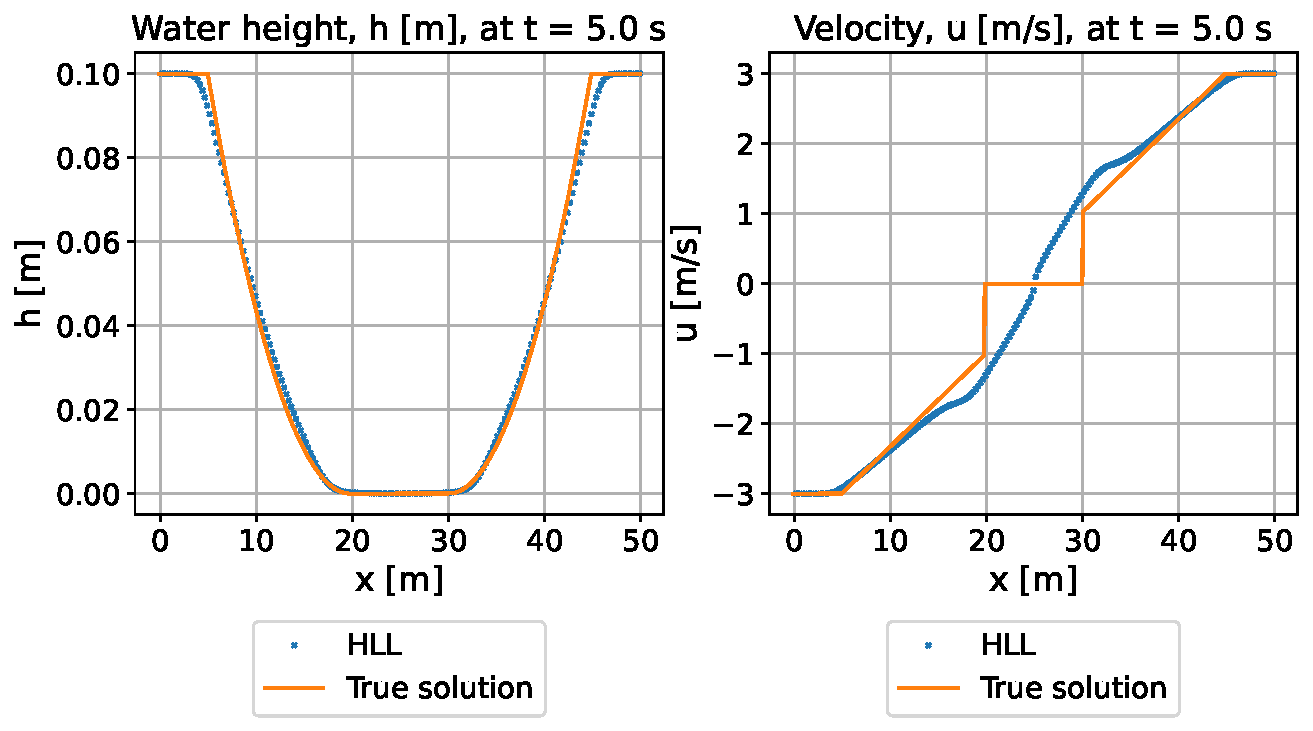
\includegraphics[width=\textwidth]{C:/Users/Matteo/Shallow-Water-Equations/plots/toro_test5_final_HLL.pdf}
        \subcaption{HLL flux.}
    \end{minipage}
    \caption{Comparison of the different fluxes for Toro test case 5.}\label{fig:toro_test5_fluxes}
\end{figure}



\newpage
\section{2D SWE long term prediction}\label{app:2D_SWE_long_term_prediction}
In this section, we present the long-term predictions for solving the 2D SWE using the CNN and FNO models.
We present the predictions for $t = 10.5$ s and $t = 12.5$ s.

The results for the long-term predictions for the CNN model for $t = 10.5$ s can be seen in \autoref{fig:2D_CNN_long_term_predictions}.
\begin{figure}[H]
    \centering
    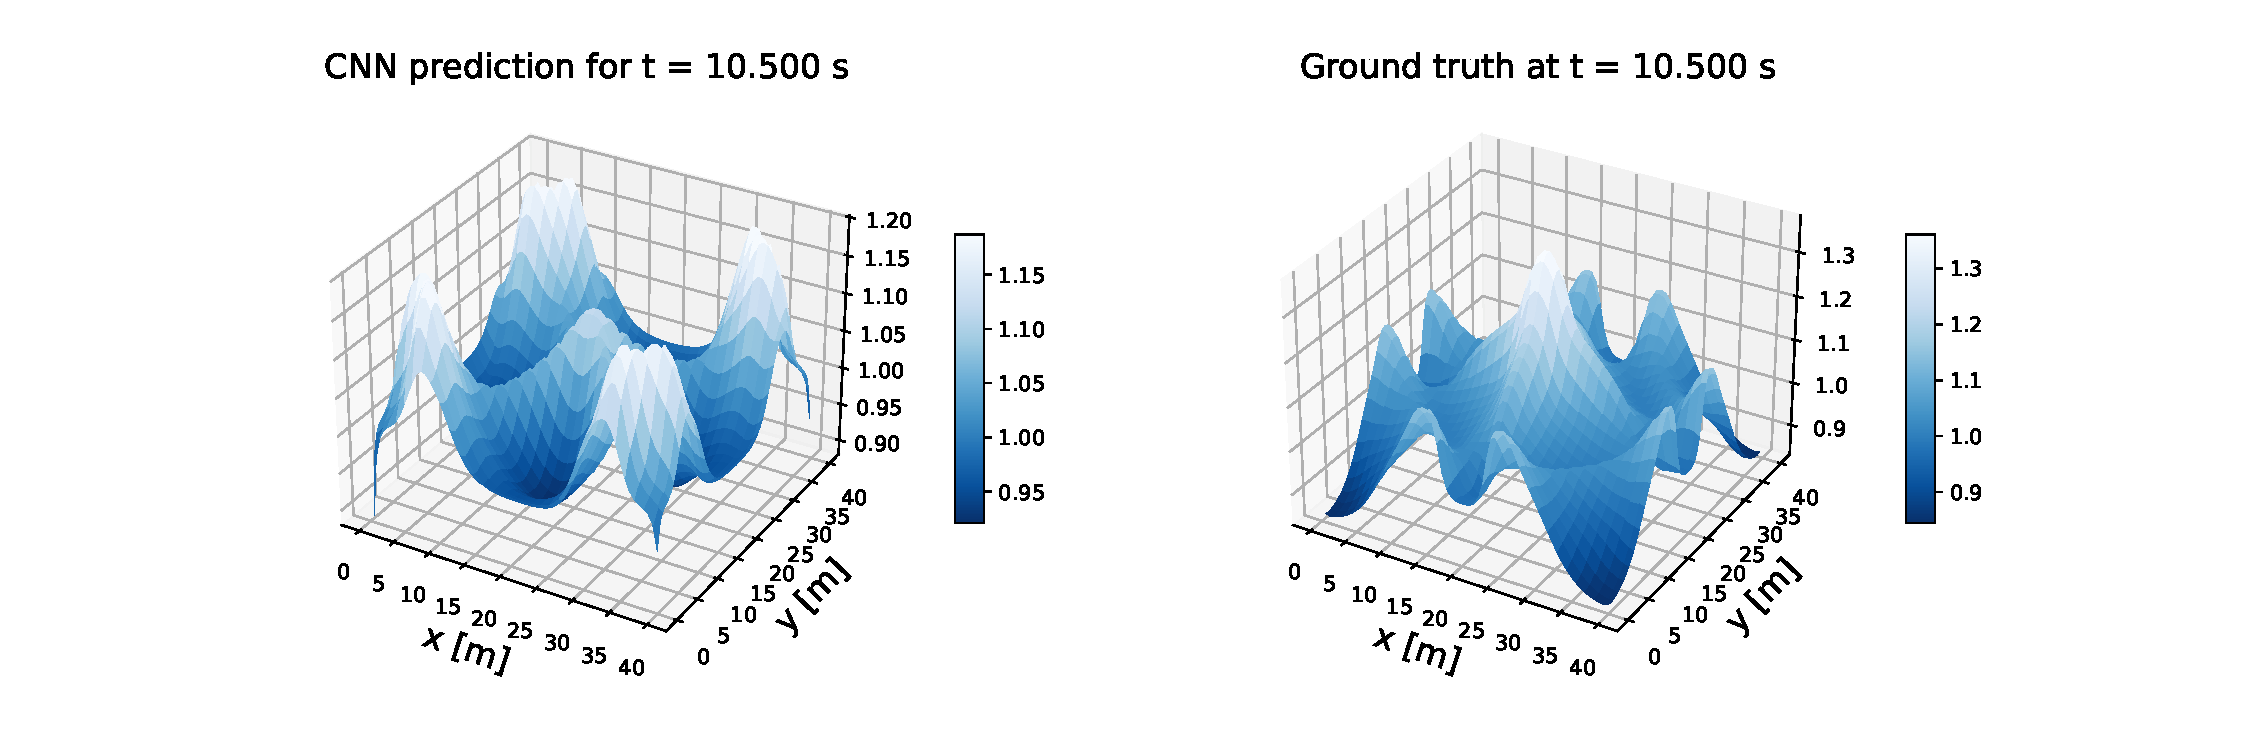
\includegraphics[width=\textwidth]{C:/Users/Matteo/Shallow-Water-Equations/plots/2D_CNN_long_term_predictions_Ntrain=64_Npred=64_idx=20.pdf}
    \caption{Long-term prediction for the 2D CNN model.}\label{fig:2D_CNN_long_term_predictions}
\end{figure}

The results for the long-term predictions for the FNO model for $t= 10.5$ s can be seen in \autoref{fig:2D_FNO_long_term_predictions}.
\begin{figure}[H]
    \centering
    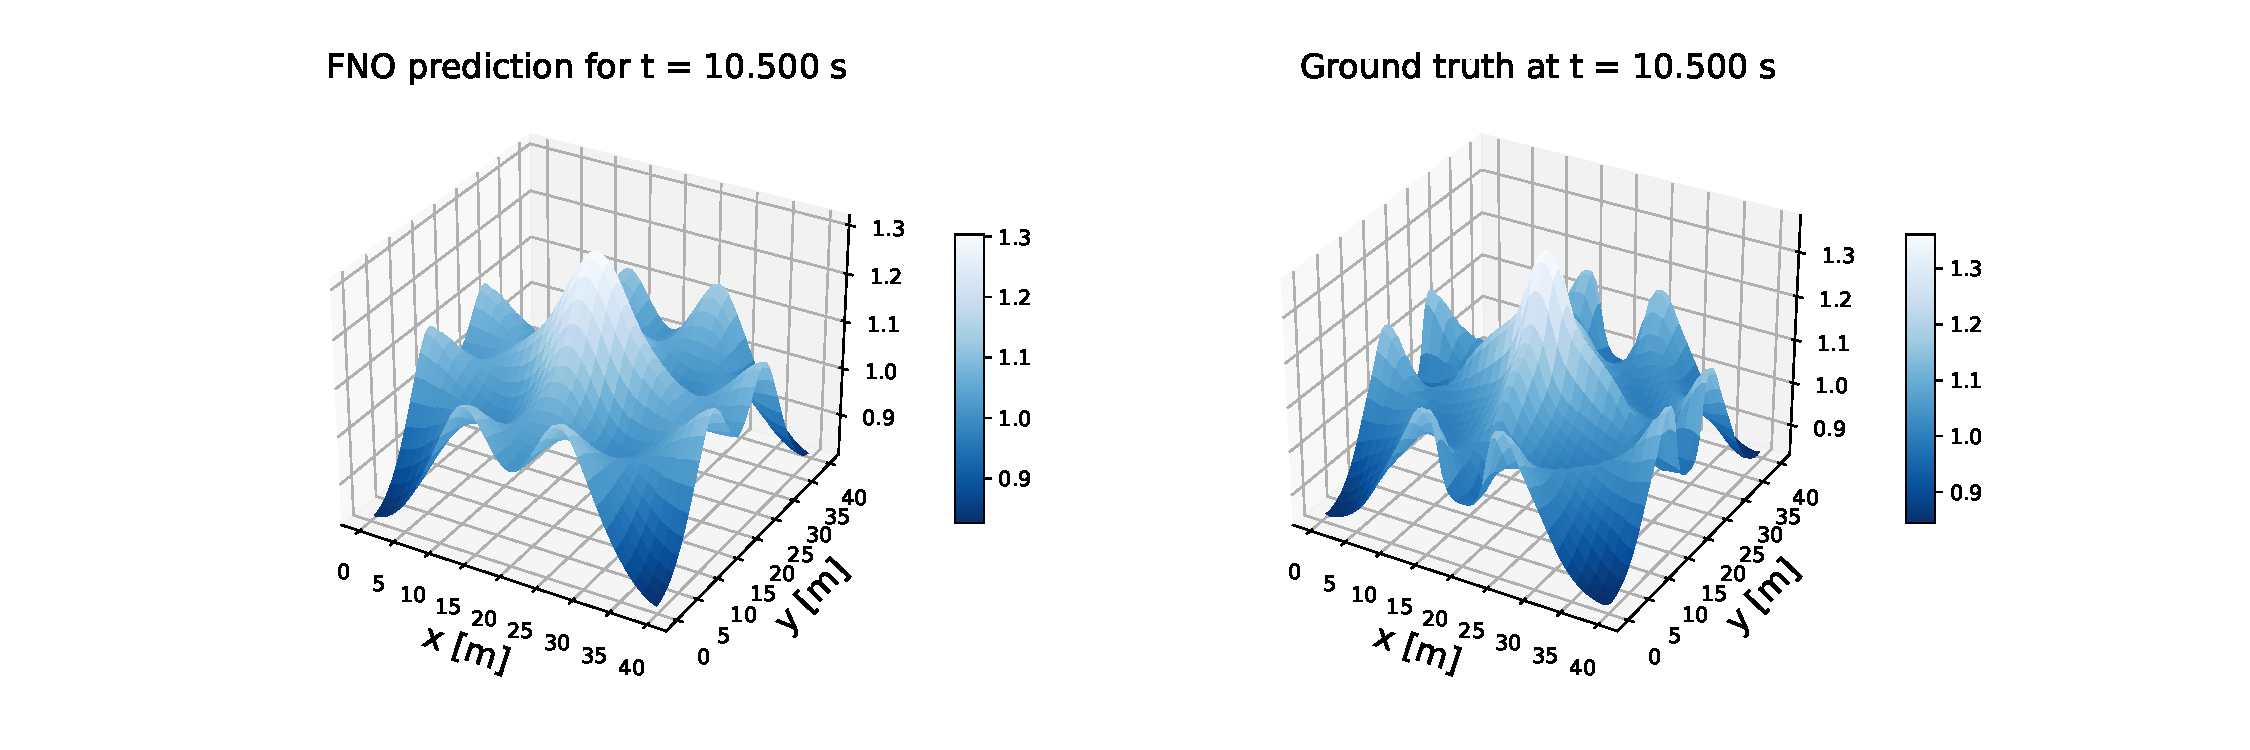
\includegraphics[width=\textwidth]{C:/Users/Matteo/Shallow-Water-Equations/plots/2D_FNO_long_term_predictions_Ntrain=64_Npred=64_idx=20.pdf}
    \caption{Long-term prediction for the 2D FNO model.}\label{fig:2D_FNO_long_term_predictions}
\end{figure}

The results for the long-term predictions for the CNN model for $t= 12.5$ s can be seen in \autoref{fig:2D_CNN_long_term_predictions_2}.
\begin{figure}[H]
    \centering
    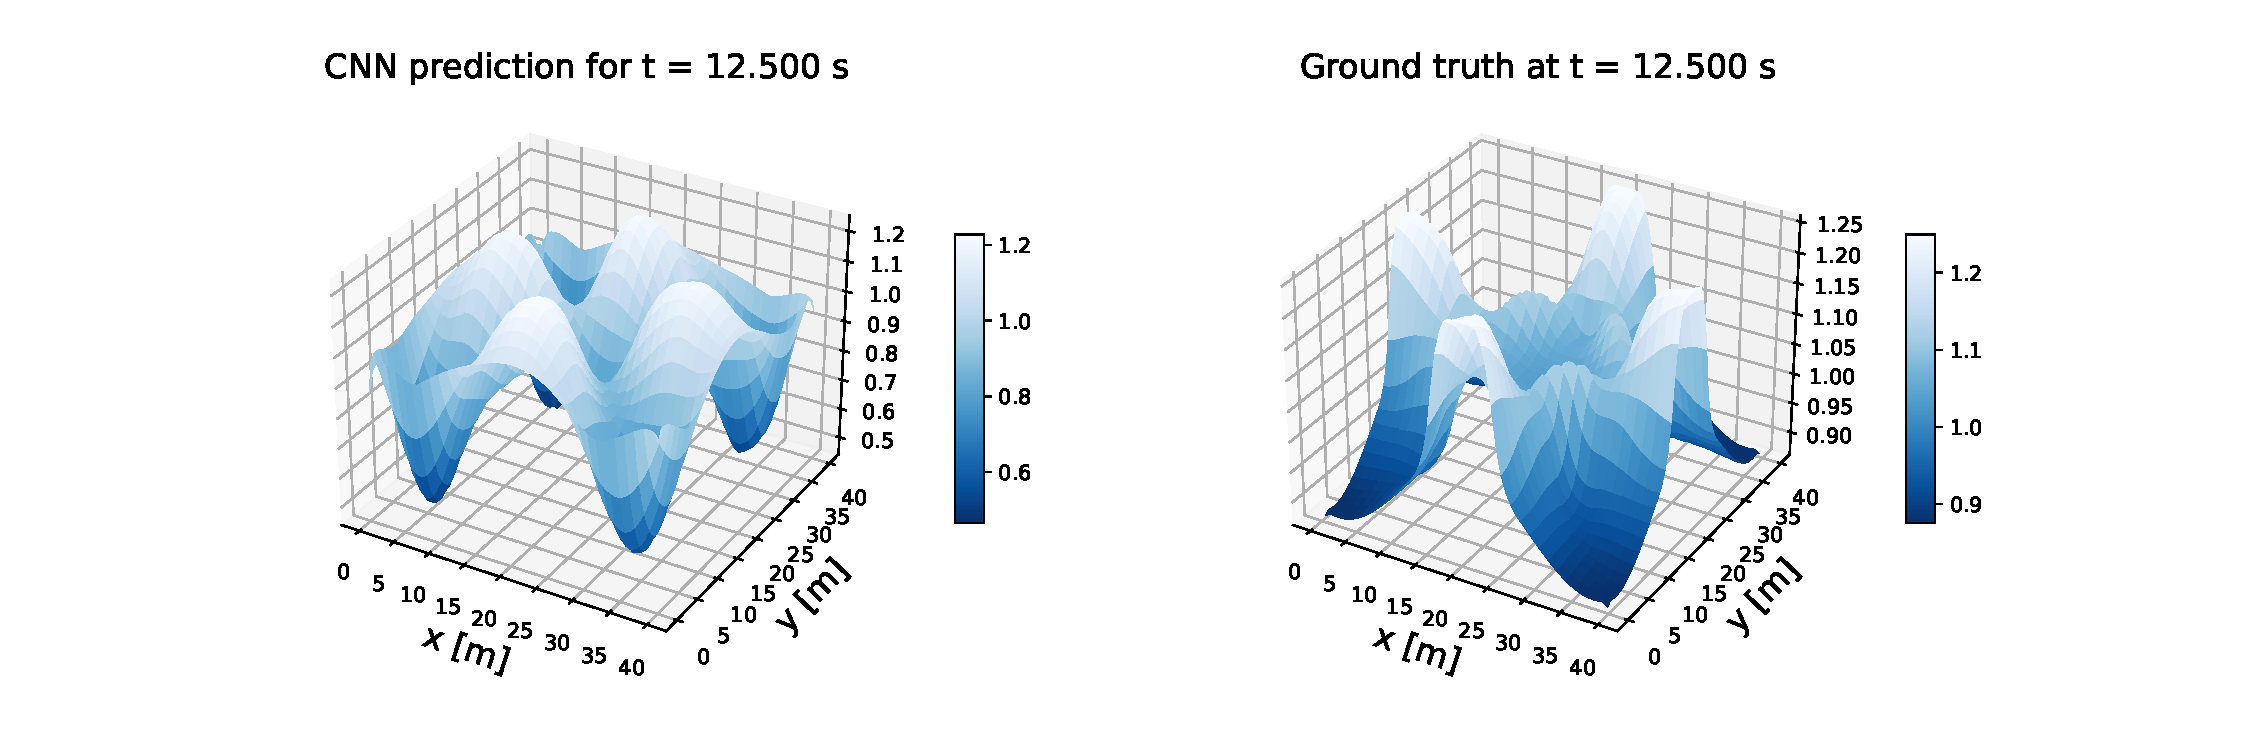
\includegraphics[width=\textwidth]{C:/Users/Matteo/Shallow-Water-Equations/plots/2D_CNN_long_term_predictions_Ntrain=64_Npred=64_idx=100.pdf}
    \caption{Long-term prediction for the 2D CNN model.}\label{fig:2D_CNN_long_term_predictions_2}
\end{figure}

The results for the long-term predictions for the FNO model for $t= 12.5$ s can be seen in \autoref{fig:2D_FNO_long_term_predictions_2}.
\begin{figure}[H]
    \centering
    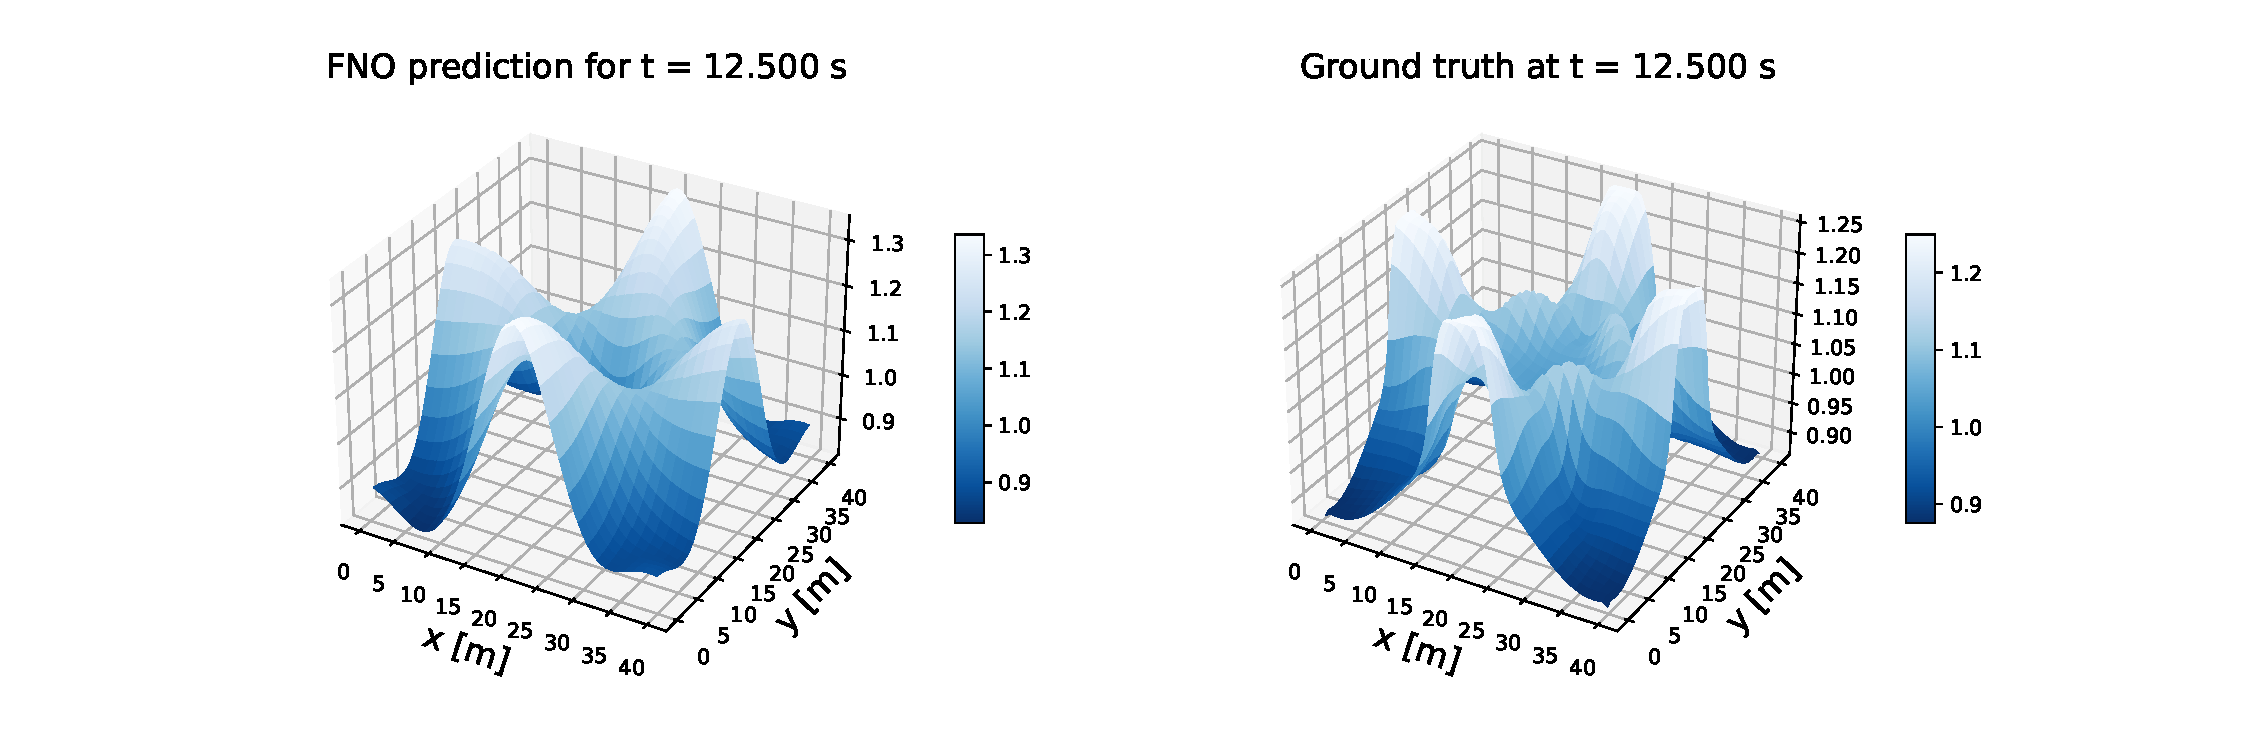
\includegraphics[width=\textwidth]{C:/Users/Matteo/Shallow-Water-Equations/plots/2D_FNO_long_term_predictions_Ntrain=64_Npred=64_idx=100.pdf}
    \caption{Long-term prediction for the 2D FNO model.}\label{fig:2D_FNO_long_term_predictions_2}
\end{figure}


\section{Code}
The code used for this project can be found at: \cite{Github_SWE}.
The animations can be found at: \url{https://github.com/MelissaJessen/Shallow-Water-Equations-Animations}.

